\documentclass[a4paper,11pt]{style-esi/td}

\usepackage{style-esi/licence}
\usepackage{style-esi/exercice}
\usepackage{style-esi/listing}
\usepackage{style-esi/tutoriel}
\usepackage{style/dev1}

\begin{document}

\seance{9}{Les tests unitaires}{td09-tests-unitaires}{
	Un code est souvent modifié, 
	cela veut dire que le temps passé à le simplifier 
	est souvent gage d’un gain de temps lors d’une modification ultérieure. 
	Il vous sera même peut-être conseillé par votre professeur de :
	faire un code fonctionnel, 
	de le modifier afin d’améliorer sa lisibilité et sa modularité
	ou, enfin, d’en améliorer son efficacité.
}

%====================
\section{Introduction}
%====================	

	La démarche que l'on vous demande de suivre dans ce TD permet d'avoir un code sans bug\footnote{Un code sans bug est difficile à obtenir, mais un développeur doit les éviter autant qu'il peut.}, grâce aux tests unitaires ainsi que le développement dirigé par les testes. Ces méthodologies permettent d'obtenir des tests maintenables tout au long de la vie d'un code.

	Jusqu'à présent, nous vous avons demandé d'écrire du code afin de répondre à une demande. Pour cela, vous avez dû~:
	\begin{enumerate}
		\item lire et comprendre l'énoncé~;
		\item déterminer les entrées et les sorties~;
		\item penser votre algorithme~;
		\item traduire l'algorithme en pseudo-code et/ou Java~;
		\item tester votre algorithme.
	\end{enumerate}

	Dans ce laboratoire, vous allez faire ce que l'on appelle du \emph{développement dirigé par les tests}. Pour faire court, il s'agit d'écrire les tests avant d'avoir écrit le code. Cela est possible car on sait, avant de l'écrire, ce que le code est censé faire.

	Ce que vous devez faire tout au long de ce TD est~:
	\begin{enumerate}
		\item lire et comprendre l'énoncé~;
		\item déterminer les entrées et les sorties~;
		\item penser aux tests que vos méthodes devront passer~;
		\item écrire les tests~;
		\item penser votre algorithme~;
		\item traduire l'algorithme en pseudo-code et/ou Java~;
		\item tester votre algorithme.
	\end{enumerate}


%====================
\section{La couverture de code}
%====================	

	Ensemble, tentons de comprendre ce qu'est une bonne \emph{couverture de code} en reprenant notre fonction valeur absolue qui est définie de la façon suivante~:
	$$
		|x| = x \textrm{ si } x \geq 0, -x \textrm{ sinon}.
	$$

	Soit la méthode \texttt{abs} qui a pour signature \code{java}{public static double abs(double x)}.

	Nous allons maintenant réfléchir aux tests que nous devons réaliser afin de garantir le bon fonctionnement de notre méthode. C'est-à-dire, les tests nécessaires\footnote{Avoir les testes nécessaires et suffisants c'est mieux. À défaut, il en vaut mieux trop que pas assez.} pour garantir le fonctionnement de la méthode quelle que soit l'entrée passée à la méthode.

	Prenons une valeur positive, 4 par exemple. Le code suivant, qui n'est pas la valeur absolue, passe avec succès notre test puisqu'il va retourner la valeur d'entrée.
	\begin{Code}{Java}
		public static double abs(double x) {
			return x;
		}
	\end{Code}


	Si l'objectif n'est pas de trouver un code pour lequel les tests fonctionnent, il montre bien que notre batterie de tests est insuffisante.

	Ajoutons un second test en essayant l'entrée $-4$. Le code suivant, qui n'est pas la valeur absolue, passe avec succès nos deux tests. 

	\begin{Code}{Java}
		public static double abs(double x) {
			return 4;
		}
	\end{Code}

	Si nous prenons toutes nos observations en considération, nous obtenons le plan de tests suivant

	\begin{center}
		\begin{tabular}{|c|c|c|c|}
			\hline
			\no du test & entrées & résultat attendu & note \\
			\hline
			1 & 4 & 4 & nombre positif \\
			\hline
			2 & -6 & 6 & Un nombre négatif \\
			\hline
		\end{tabular}
	\end{center}

	Même si notre exemple est aberrant, nous souhaitons ici mettre en évidence la difficulté d'obtenir des tests complets, que le processus d’élaboration des tests unitaires demande de la réflexion et qu’il ne garantit pas à 100\% le bon fonctionnement du code. Il est donc essentiel de prendre le temps nécessaire afin de fournir une couverture de code aussi complète et exacte que possible\footnote{Vous pouvez remarquer que pour chacun de nos exemples, la couverture de code est de 100\% ; et que malgré cela, le code ne fait pas toujours ce qu'on souhaitait qu'il fasse.}.

	\begin{Exercice}{Max - Couverture de code}
		Donnez les entrées et sorties nécessaires à l’élaboration d’une bonne couverture de code pour la méthode \code{java}{max(int a, int b)} qui permet d’obtenir la plus grande valeur parmi les~2 passées en paramètre.
	\end{Exercice}

	\begin{Exercice}{Somme d'entiers consécutifs - Couverture de code}
		
		Donnez les entrées et sorties nécessaires à l’élaboration d’une bonne couverture de code pour la méthode \code{java}{somme(int n)}. Cette méthode calcule la somme des entiers consécutifs de 1 à n.
	\end{Exercice}

	\begin{Exercice}{Anagramme - Couverture de code}
		\og Une anagramme est une construction fondée sur une figure de style qui inverse ou permute les lettres d’un mot ou d’un groupe de mots pour en extraire un sens ou un mot nouveau.\fg Wikipedia.\footnote{https ://fr.wikipedia.org/wiki/Anagramme}. 

		Donnez les entrées et sorties nécessaires à l’élaboration d’une bonne couverture de code de la méthode \code{java}{boolean estAnagramme(String mot, String candidat)}. Cette méthode vérifie si une chaîne de caractères est un anagramme.
	\end{Exercice}

	\begin{Exercice}{Palindrome - Couverture de code}
		\og Le palindrome est un texte ou un mot qui reste identique qu’on le lise de gauche à droite ou de droite à gauche. Nous considérons ici la version stricte dans le sens où l’on prend en considération les signes diacritiques (accents, trémas, cédilles) ainsi que les espaces.\fg Wikipedia\footnote{https ://fr.wikipedia.org/wiki/Palindrome}.

		Donnez les entrées et sorties nécessaires à l’élaboration d’une bonne couverture de code de la méthode \code{java}{boolean estPalindrome(String mot, String candidat)}. Cette méthode vérifie qu'un texte est un palindrome.
	\end{Exercice}

	\begin{Exercice}{Nombre occurrences - Couverture de code}
		Donnez les entrées et sorties nécessaires à l’élaboration d’une bonne couverture de code de la méthode \code{java}{public static int nbOccurance(char lettre, String texte)}. Cette méthode permet de compter le nombre d'occurrences d’une lettre dans un texte.
	\end{Exercice}

%====================
\section{JUnit}
%====================

	Si nous reprenons l’exemple de la méthode calculant la valeur absolue, nous pourrions la développer et la tester comme ceci :
	\listing[basicstyle=\footnotesize\vtt]{java}{MonMath.java}

	Au lancement du code, les deux tests passent.
	\begin{Console}
		abs(4) = 4 ? true
		abs(-6) = 6 ? true
	\end{Console}

	Les problèmes avec cette méthodologie sont multiples.
	\begin{enumerate}
		\item Il ne peut y avoir qu’une seule méthode main par fichier Java.
 		\item On doit avoir accès au fichier pour compléter les tests.
 		\item Il faut être rigoureux pour que les tests soient lisibles.
 		\item Le lancement des tests peut prendre du temps puisqu'il faut lancer chaque fichier séparément...
	\end{enumerate}
	Tous ces problèmes mènes à un problème de maintenabilité des tests et du code.

	Notre manière de tester peut être améliorée en sortant les méthodes principales dans des fichiers différents et le dernier point en mettant tous les tests dans la même méthode, mais il nous reste à être rigoureux pour obtenir un code maintenable. Nous allons donc utiliser le framework JUnit qui va nous permettre d'obtenir cette lisibilité.

	La première chose à faire est de configurer Netbeans. Heureusement pour vous, il fait presque tout lui même (à condition de bien s’y prendre).
	Après avoir écrit le fichier \bsc{MonMath.java} dans un nouveau package \bsc{esi.dev1.td9}, faite un clique droit sur le package. Sélectionnez tools et faite Create/Update tests.

	\begin{center}
		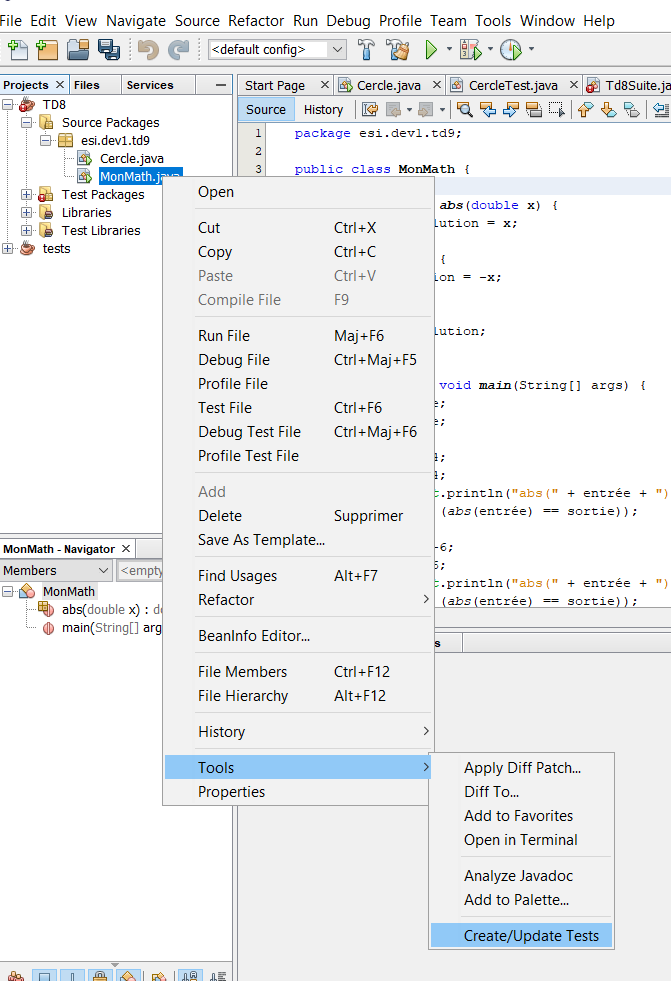
\includegraphics[width=.4\textwidth]{images/create_tests}
	\end{center}


	Une nouvelle fenêtre va apparaître, décochez les 4 checkbox en dessous de \og Generated Code\fg et validez. 

	\begin{center}
		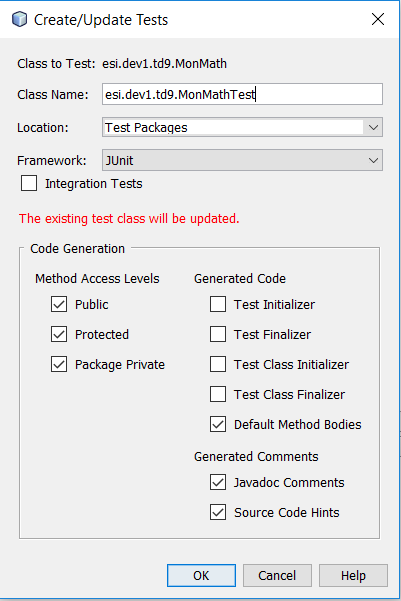
\includegraphics[width=.3\textwidth]{images/config_tests}
	\end{center}

	De nouveaux éléments, créés par NetBeans, apparaissent dans votre projet. D’une part les librairies utilisées par NetBeans ainsi qu’un nouveau dossier nommé Tests packages. Dans ce dossier se trouver une nouvelle classe \bsc{MonMathTest.java}. C'est dans cette classe que vous écrirez vos premiers tests.

	\begin{center}
		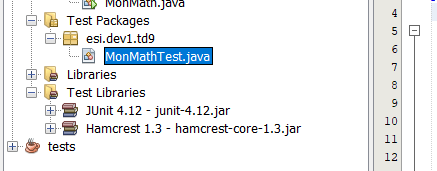
\includegraphics[width=.4\textwidth]{images/libraries}
	\end{center}

	Il vous reste à considérer le message laissé par netbeans.
	\begin{Code}{Java}
		// TODO review the generated test code and remove the default call to fail.
	\end{Code}

	Une fois le code nettoyé, vous devriez obtenir ceci~:
	\listing{java}{MonMathTestEMPTY}

	La variable x représente l’entrée de la méthode à tester et la variable \texttt{expResult} représente le résultat attendu.

	La méthode \texttt{asserEquals} est une méthode qui prend en paramètre :
	\begin{itemize}
		\item Le résultat attendu.
		\item Le résultat obtenu (calculé par la méthode que vous souhaitez tester).
		\item Une marge d’erreur.
	\end{itemize}

	Le troisième paramètre ne doit être utilisé que si la sortie de la méthode est de type double \footnote{Pourquoi ?}.
	L’appel à la méthode \texttt{assertEquals} avec un retour de méthode entier s’écrit donc :
	\code{java}{assertEquals(expResult, result)}.
	Si la méthode que vous testez retourne un booléen, il est alors préférable d’utiliser les méthodes \texttt{assertTrue} ou \texttt{assertFalse}. Ces méthodes prennent un unique paramètre, le résultat, puisque le résultat attendu est défini par la méthode qu'on a choisi d'utiliser. En effet en utilisant \texttt{assertTrue}, on s’attend à avoir une expression évaluée à \bsc{true}.

	\subsection{Tester le lancement d'une exception}
	%=============================
	Si nous reprenons le code de la méthode périmètre, nous remarquons qu'une exception est lancée dans le cas d'un rayon négatif. En effet, notre plan de test doit ressembler à quelque chose comme ceci~:

	\begin{center}
		\begin{tabular}{|c|c|c|c|}
			\hline
			\no du test & entrées & résultat attendu & note \\
			\hline
			1 & 0 & 0 & Extremum du domaine de définition \\
			\hline
			2 & 4 & 25.12 & valeur positive (précision 0.01) \\
			\hline
			3 & -5 & \texttt{erreur} & valeur négative \\
			\hline
		\end{tabular}
	\end{center}

	Nous vous laissons réaliser les deux premiers tests. Pour vérifier le lancement d'une exception, ajoutez le tag \texttt{@Test} en spécifiant le type de l'exception attendue.
	\listing{java}{CercleTest.java}

	Remarquez que dans le cas présent, vous ne devez pas ajouter de méthode \texttt{assert}\footnote{Pourquoi ?}.

	\begin{Exercice}{Couverture de code - Exceptions}
		Pour chacun des exercices précédents, vérifiez que vous avez bien pensé aux cas menant à des erreurs.
	\end{Exercice}

	\begin{Exercice}{Implémentation - Max}
		\vspace{-1em}
		\begin{enumerate}
			\item Dans le fichier MonMath, ajoutez la signature de la méthode \texttt{max}. Faite un retour quelconque afin de rendre le code compilable.
			\item Développez, avec le framwork JUnit, votre couverture de code écrite précédemment.
			\item Lancez votre fichier de test.
			\item Développez votre méthode afin que celle-ci complète tous les tests.
		\end{enumerate}
	\end{Exercice}

	\begin{Exercice}{Implémentation - Somme d'entiers consécutifs}
		\vspace{-1em}
		\begin{enumerate}
			\item Dans le fichier MonMath, ajoutez la signature de la méthode \texttt{somme}. Faite un retour quelconque afin de rendre le code compilable.
			\item Développez, avec le framwork JUnit, votre couverture de code écrite précédemment.
			\item Lancez votre fichier de test.
			\item Développez votre méthode afin que celle-ci complète tous les tests.
		\end{enumerate}
	\end{Exercice}
	
	\newpage 
	
	\begin{Exercice}{Implémentation - Anagramme}
		\vspace{-1em}
		\begin{enumerate}
			\item Dans le fichier MesMots, ajoutez la signature de la méthode \texttt{estAnagramme}. Faite un retour quelconque afin de rendre le code compilable.
			\item Développez, avec le framwork JUnit, votre couverture de code écrite précédemment.
			\item Lancez votre fichier de test.
			\item Développez votre méthode afin que celle-ci complète tous les tests.
		\end{enumerate}
	\end{Exercice}

	\begin{Exercice}{Implémentation - Palindrome}
		\vspace{-1em}
		\begin{enumerate}
			\item Dans le fichier MesMots, ajoutez la signature de la méthode \texttt{estPalindrome}. Faite un retour quelconque afin de rendre le code compilable.
			\item Développez, avec le framwork JUnit, votre couverture de code écrite précédemment.
			\item Lancez votre fichier de test.
			\item Développez votre méthode afin que celle-ci complète tous les tests.
		\end{enumerate}
	\end{Exercice}

	\begin{Exercice}{Implémentation - Nombre d’occurrences}
		\vspace{-1em}
		\begin{enumerate}
			\item Dans le fichier MesMots, ajoutez la signature de la méthode \texttt{nbOccurances}. Faite un retour quelconque afin de rendre le code compilable.
			\item Développez, avec le framwork JUnit, votre couverture de code écrite précédemment.
			\item Lancez votre fichier de test.
			\item Développez votre méthode afin que celle-ci complète tous les tests.
		\end{enumerate}
		
	\end{Exercice}




%====================
\section{Exercices supplémentaires}
%====================	
	\begin{Exercice}{Implémentation - PGCD}
		Selon le principe TDD, implémentez la méthode \code{java}{pgcd(int a, int b)} qui retourne le pgcd de deux nombres.
	\end{Exercice}

	\begin{Exercice}{Implémentation - PPCM}
		Selon le principe TDD, implémentez la méthode \code{java}{ppcm(int a, int b)} qui retourne le ppcm de deux nombres.
	\end{Exercice}

	\begin{Exercice}{Implémentation - Chiffrement par décalage}
		Selon le principe TDD, implémentez la méthode \code{java}{césar(String texte, int décalage)} qui permet de retourner un texte chiffré selon le code de César%
		\footnote{%
			\url{https ://fr.wikipedia.org/wiki/Chiffrement\_par\_d\%C3\%A9calage}
		}.
		
	\end{Exercice}


\end{document}